\documentclass{article}

\usepackage[utf8]{inputenc}
\usepackage[francais]{babel}
\usepackage{dirtree}
\usepackage{graphicx}
\usepackage{float}

% elements du titre
\title{Rapport projet 2, TSAT - Solveur SAT/SMT}
\author{T. Stérin, A. Torres}
\date{Mai 2016}


% definition de quelques macros, pour les maths
\newcommand{\litt}{\alpha}
\newcommand{\non}[1]{\overline{#1}}

\begin{document}

\maketitle

\begin{abstract}
Réalisé à l'ENS Lyon pour l'année scolaire 2015-2016 et dans le cadre de la matière ``Projet2'' TSAT est un solveur SAT/SMT à l'instar de minisat \cite{minisat} qui a pour but de satisfaire des formules logiques qui lui sont données en entrée.
TSAT est écrit en C++ par Tristan Stérin et Alexy Torres--Aurora-Dugo.
Différentes méthode de résolution ont été implémentées dans TSAT : 
\begin{itemize}
	\item DPLL (Davis–Putnam–Logemann–Loveland) standard \cite{DPLL}.
	\item DPLL avec méthode des litéraux surveillés \cite{WL}.
	\item DPLL avec méthode avec apprentissage de clause \cite{CL}.
	\item DPLL(T) dans le cadre SMT avec les théories de l'égalité, de la congruence \cite{SMT}. 
\end{itemize}
\end{abstract}
%Un peu de maths en \LaTeX: voici un exemple de clause:
%$$
%\litt_1\lor\non{\litt_2}\lor\litt_4
%$$
%On remarque au passage que $\non{\non{\litt}}$ est pareil que $\litt$.

\section{Organisation du code}
L'organisation du projet est la suivante :
\dirtree{%
    .1 src/.
    .2 BETHeuristic (Classes contenant les stratégies de pari).
    .2 Global (Fichiers source contenant les paramètres du programme).
    .2 Core (Noyau TSAT, structures de clause).
    .3 SMT (Noyau SMT).
    .2 Parser (Parseurs CNF et logique).
    .2 RandomSatExpGenerator (Générateur de formules SAT).
    .2 SMTGenerator (FGénérateur de formules SMT).
    .2 main.cpp (Fichier source principal du solveur).
    .2 main.h (En tête du fichier main.cpp).
    .2 Makefile (Fichier de compilation du solveur).
}
\newpage

\section{Résumé des features}
\subsection{SAT}
\begin{itemize}
\item Gestions des formules au format DIMACS/FOR.
\item DPPL standard, Watched Literals, Clause Learning avec interaction possible.
\item Heuristiques : RAND, MOMS, DLIS, VSIDS.
\item Génération de formules aléatoires.
\end{itemize}

\subsection{SMT}
\begin{itemize}
\item Égalité \textbf{avec clause learning SMT}.
\item Congruence (QF UF) \textbf{sans clause learning SMT}.
\item Possibilité de désactiver le clause learning SMT pour comparer les performances (-disable\_smt\_cl).
\item Génération de formules aléatoires.
\end{itemize}
\subsection{SMT}

\section{Choix d'implémentation}
Le patron de conception en statégies à été retenu pour le développement des heuristiques de pari. Cela permet d'ajouter une heuristique sans modifier le noyau SAT. 
Cette méthode de conception permettrait aussi de modifier l'heuristique de pari durant le traitement de la formule.

Nous avons aussi développé les différents parseurs de formule à l'aide de ce patron de conception afin de faciliter l'ajout de nouveaux types de parseurs.

Les théories de l'égalité et de la congruence ont une formulation proche, nous aons donc utilisé la même base de code pour les traiter.
Elles utilisent toutes deux un union find codé séparément en tant qu'outil.

Cela a beaucoup évolué au cours du projet. Nous avons trouvé d'ailleurs que c'était l'une des difficultés du cours : faire une architecture assez maléable pour intégrer facilement des ajouts futurs. En pratique nous avons souvent ré-écrit tout le code (3 fois).
L'architecture finale se veut la plus simple possible avec une utilisation massive d'unordered set et d'unordered map.

\section{Détection de l'UIP}
Nous avons implémenté un algorithme linéaire trouvé pour l'occasion. Étant donné un DAG à une source et un puit on souhaite trouver les noeuds tels que tous les chemins de la source au puit passe par eux : les UIP. On cherche plus particulièrement celui qui est le plus proche du puit.
On s'appuie sur la remarque suivante : tous les UIP sont sur le plus court chemin entre la source et le puit. \\
Nous sommes dans un cas particulier où le puit a exactement deux pères. Pour ces deux noeuds on calcule le plus haut noeud du plus court chemin auquel il peut remonter sans passer par les arêtes du plus court chemin. Le plus haut des deux est le 1-UIP. Cet algorithme est linéaire.

\section{Critique des performances}
\subsection{SAT}
La méthode avec apprentissage de clause permet d'obtenir de très bons résultats.

Pour les heuristiques, les meilleurs résultats s'obtiennent avec l'heuristique MOMS.

Les optimisations à la compilation (-O3) permettent elles aussi de rendre le solveur beaucoup plus rapide (jusqu'à 70\% plus rapide dans certain cas).
\\
\begin{figure}[h]
    \begin{center}
        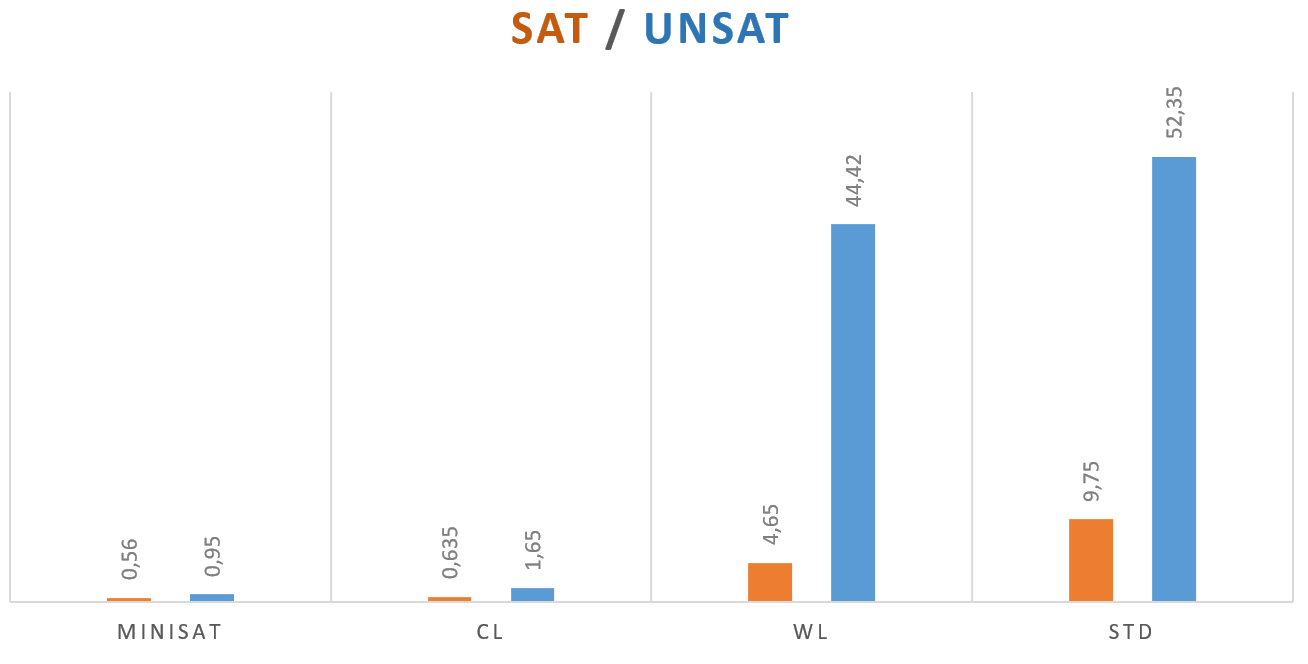
\includegraphics[scale=0.25]{time.png}
    \end{center}
    \caption{Comparaison des temps d'execution de TSAT à MINISAT}
    \label{Comparaisons}
\end{figure}

\subsection{SMT}
Dans le cadre de l'égalité on propose de désactiver l'apprentissage de clause SMT. On constate par exemple sur le test gros.for l'efficacité de l'apprentissage SMT. Ce test est résolu en 15s avec apprentissage SMT et ne termine pas sans.

\subsection{Remarques SMT}

En cas de satisfiabilité SMT le solveur renvoie : 
\begin{itemize}
\item Égalité : un nombre minimal de classes d'équivalences incompatibles.
\item QF UF : un nombre minimal de classes d'équivalences de termes incompatibles. On prend en compte ici tous les termes qui apparaissent dans la formule (y compris les sous termes).

\end{itemize}

\section{Améliorations possible}
Plusieurs possibilités d'améliorations sont envisageables : 
\begin{itemize}
\item Une parallélisation des tâches pourrait faire gagner du temps. On pourrait par exemple exécuter en même temps différentes heuristiques de pari sur la prochaine variable à assigner.
\item Il faudrait implémenter le clause learning pour la congruence décrit dans \cite{SMT}.
\item Le code pourrait être encore allégé, mais encore une fois, on s'en rend compte toujours après l'avoir écrit!
\end{itemize}

\bibliographystyle{unsrt}
\bibliography{ex-biblio}

\end{document}
